Para decorar um cilindro circular reto ser� usada uma faixa retangular de papel transparente, na qual est� desenhada em negrito uma diagonal que forma 30� com a 
borda inferior. O raio da base do cilindro mede $\frac 6 \pi$ cm, e ao 
enrolar a faixa obt�m-se uma linha em formato de h�lice, como na figura. 

\begin{figure}[h]
\centering
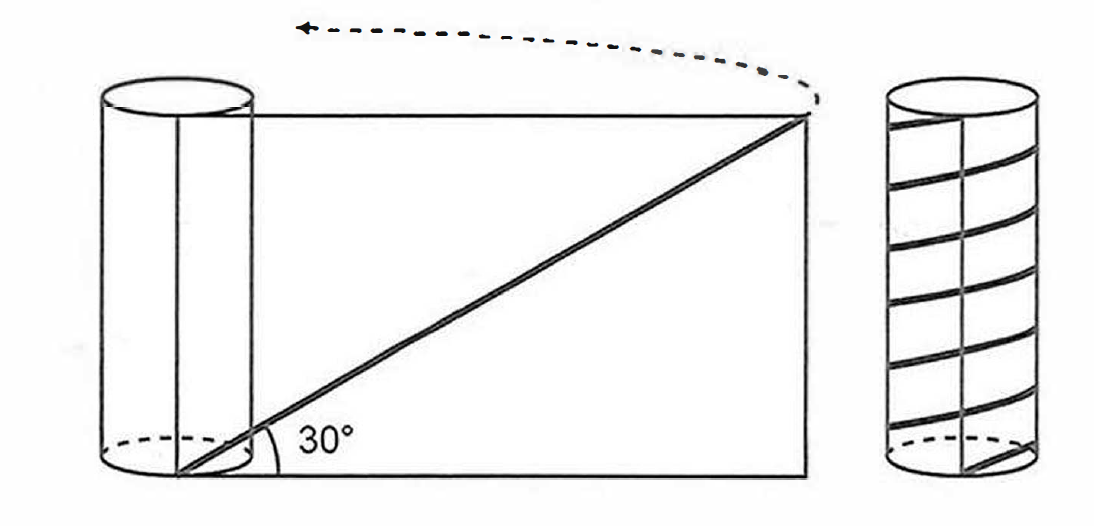
\includegraphics[width=8cm]{../figuras/q176-2018.png}
\end{figure}

O valor da medida da altura do cilindro, em cent�metro, �

\begin{enumerate}
\item[a)]$36\sqrt{3}$
\item[b)]$24\sqrt{3}$
\item[c)]$4\sqrt{3} $
\item[d)]36
\item[e)]72
\end{enumerate}